\documentclass[10pt]{article}
\usepackage{tabularx,graphicx,layout}
\usepackage{hyperref}

\begin{document}
% 
% Name of file: coo.tex
% Orignal Authors 1999 Elton Smith
%                      David Mack
%                      Javier Gomez
% Minor Updates In 2014 for 12GeV
%                      Douglas Higinbotham
%                       
% Instructions for use (Replace '*' by A, B or C):
%
% 1. Edit input tex files
%    a) coo_hall*_defs.tex
%    b) coo_hall*_appendix.tex 
% 2. Prepare Organization Chart
%    a) Modify coo_Hall*org.fig using UNIX xfig program
%    b) Export file to encapsulated postscript
% 3. Edit this file 
%    a) Select coo_hall*_defs.tex definitions (immediately following)
%    b) Select coo_Hall*org.eps input file (search down)
%    c) Select coo_hall*_appendix.tex input file (bottom of this file)
% 4. Produce Output using latex/dvips.
%
%\input{coo_hallb_defs.tex}
%\input{coo_hallc_defs.tex}
%
% sample coo_halla_defs.tex
%
%
% Hall A definitions for Standard COO input
% 
% Instructions for use of standard latex coo (Replace '*' by A, B or C):
%
% 1. Edit input tex files
%    a) coo_hall*_defs.tex
% 2. Prepare Organization Chart
%    a) Modify coo_Hall*org.fig using UNIX xfig program
%    b) Export file to encapsulated postscript
%    b) coo_hall*_checklists.tex 
% 3. Edit this file 
%    a) Select coo_hall*_defs.tex definitions (immediately following)
%    b) Select coo_Hall*org.eps input file (search down)
%    c) Select coo_hall*_checklists.tex input file (bottom of this file)
% 4. Produce Output using latex/dvips.
%
%% 
% Instructions for use of standard latex coo (Replace '*' by A, B or C):
%
% 1. Edit input tex files
%    a) coo_hall*_defs.tex
% 2. Prepare Organization Chart
%    a) Modify coo_Hall*org.fig using UNIX xfig program
%    b) Export file to encapsulated postscript
%    b) coo_hall*_checklists.tex 
% 3. Edit this file 
%    a) Select coo_hall*_defs.tex definitions (immediately following)
%    b) Select coo_Hall*org.eps input file (search down)
%    c) Select coo_hall*_checklists.tex input file (bottom of this file)
% 4. Produce Output using latex/dvips.
%
%% 
% Instructions for use of standard latex coo (Replace '*' by A, B or C):
%
% 1. Edit input tex files
%    a) coo_hall*_defs.tex
% 2. Prepare Organization Chart
%    a) Modify coo_Hall*org.fig using UNIX xfig program
%    b) Export file to encapsulated postscript
%    b) coo_hall*_checklists.tex 
% 3. Edit this file 
%    a) Select coo_hall*_defs.tex definitions (immediately following)
%    b) Select coo_Hall*org.eps input file (search down)
%    c) Select coo_hall*_checklists.tex input file (bottom of this file)
% 4. Produce Output using latex/dvips.
%
%\input{coo_halla_defs.tex}
%%
% Hall A definitions for Standard COO input
%
\def\HALL{Hall A}
\def\EXPTS{Triton Experiments}
\def\HALLLEADER{Thia Keppel}
\def\ACCDIVLIAISON{Hari Areti} 
\def\PHYSDIVLIAISON{Bob Michaels}
\def\PHYSDIVLIAISONEMAIL{rom@jlab.org} 
\def\AWARENESS{SAF110}
\def\FAMILIARITY{SAF120}

% Hall A Accelerator Physics Liaison
\def\AccPhysLiaison{Yves Roblin}

% for the other Halls
% Hall B 
% Michael Tiefenback
% Hall C
% Jay Bensesch
% Hall D
% Todd Satogata



%%
% Hall A definitions for Standard COO input
%
\def\HALL{Hall A}
\def\EXPTS{Triton Experiments}
\def\HALLLEADER{Thia Keppel}
\def\ACCDIVLIAISON{Hari Areti} 
\def\PHYSDIVLIAISON{Bob Michaels}
\def\PHYSDIVLIAISONEMAIL{rom@jlab.org} 
\def\AWARENESS{SAF110}
\def\FAMILIARITY{SAF120}

% Hall A Accelerator Physics Liaison
\def\AccPhysLiaison{Yves Roblin}

% for the other Halls
% Hall B 
% Michael Tiefenback
% Hall C
% Jay Bensesch
% Hall D
% Todd Satogata



%%
% Hall A definitions for Standard COO input
%
\def\HALL{Hall A}
\def\EXPTS{Triton Experiments}
\def\HALLLEADER{Thia Keppel}
\def\ACCDIVLIAISON{Hari Areti} 
\def\PHYSDIVLIAISON{Bob Michaels}
\def\PHYSDIVLIAISONEMAIL{rom@jlab.org} 
\def\AWARENESS{SAF110}
\def\FAMILIARITY{SAF120}

% Hall A Accelerator Physics Liaison
\def\AccPhysLiaison{Yves Roblin}

% for the other Halls
% Hall B 
% Michael Tiefenback
% Hall C
% Jay Bensesch
% Hall D
% Todd Satogata




\begin{center}
\Large 
Conduct of Operations for \HALL\ \\
\EXPTS\ \\
\today 
  
\end{center}
\normalsize

\tableofcontents


%******************************************************************************
\newpage

%\vskip0.2in 
%\noindent
%{\bf\Large{Preface}}
%\vskip0.2in 
\section{Preface}

As part of its mission, JLab provides the resources necessary for international
collaborations of scientists to carry out basic research in nuclear physics 
and related disciplines. This research must be conducted
in a manner that ensures that environmental, health and safety (EH\&S) 
concerns receive the highest consideration. At the same time the programmatic 
goals of the laboratory require that it produce the highest quality physics 
results efficiently.

Guidance on how to balance thoughtful, measured EH\&S concerns with efficient
operation has been taken from 
%the Department of Energy (DOE) Order 5480.10, ``Conduct of Operations," 
the Director's Safety Council, the JLab EH\&S Manual, and the
JLab Director's Office. A graded approach is followed in which the measures 
taken are matched to the scale, cost, complexity, and hazards of the operation.

{\bf This document outlines how approved experiment collaborations will conduct
operations in a safe and effective manner during the time period that 
\EXPTS\  is on the floor. Installation 
periods are not covered by this document. 
Furthermore, this document is directed to physics users and
physics staff rather than the \HALL\ technical staff.  It must be read, 
understood, and followed by all members of the collaboration. }

%******************************************************************************
\section{Documentation}

This experiment uses the standard \HALL\ equipment. 
All of the procedures to be used during the course of the experiment are contained in the following
documents\footnote{The process is documented at \url{http://www.jlab.org/user_resources/PFX} }:

%\begin{description}
\begin{itemize}

\item  The Conduct of Operations for \HALL\ \EXPTS\
 (COO), the document you are now reading. 

\item   Experiment Safety Assessment Document (ESAD)
for \EXPTS\ (referring to the base equipment as well as any 
experiment-specific changes)

\item Radiation Safety Assessment Document (RSAD) 

\item JLab Emergency Response Guidelines (ERG) 

\item \HALL\ Standard Equipment Manual 

\end{itemize}

%\end{description}

Reference copies of these documents will be available in the Counting 
House for the duration of the experiment. The present document shall 
hereafter be referred to as the COO. The Experiment Safety Assessment 
Document shall hereafter be referred to as the ESAD, and the
Radiation Safety Assessment Document shall be referred to as the RSAD.
The ESAD and COO may also be available on the WWW at an experiment-specific 
web site. {\bf The COO, the ESAD and the RSAD are required reading for 
shift personnel.}

A full description of the physics motivation for the experiments, collaboration 
lists, and general plans for carrying out an experiment can be found in the
proposal(s) to the JLab Program Advisory Committee (PAC). 

%******************************************************************************
\section{Shift Personnel Training}

All personnel on shift are required to have successfully completed and be 
current in the following JLab safety training:

\begin{itemize}

\item EH\&S Orientation (SAF 100) 

\item Radiation Worker Training (SAF 801) 

\item Oxygen Deficiency Hazard Training (SAF 103) 

\item \HALL\ Safety Awareness Walk-Through ( \AWARENESS\ )

\end{itemize}

 All experiment personnel are 
required to have radiation badges in their possession during their shifts. 
The Safety Awareness Walk-Through will
emphasize hazards that are typical of normal Hall operations.
Hazards  peculiar to the current experimental setup are addressed in the appendices 
of this document. 
In addition, all shift personnel will be trained in the safety procedures to be
followed for access to the Hall. This
training will include a brief discussion of the purpose and operation of the
Personnel Safety System (PSS) for the Hall. 
Individuals within the collaboration may be required to have other equipment 
or procedure-specific training. The need for such
training shall be determined by the experiment spokesperson in consultation 
with the Hall Leader and Physics Division Safety Officer.

In addition, experiment personnel must familiarize themselves with the 
sections of the JLab EH\&S Manual relevant for their work in the Hall. 
A reference copy of this
document is available in the main hallway of the Counting House. It is also
available via \url{http://www.jlab.org/ehs/ehsmanual/index.html}.

Finally, JLab Lock and Tag\footnote{The EH\&S Manual provides Lockout/Tagout
information in Chapter 6110 at \url{http://www.jlab.org/ehs/ehsmanual/manual6110.html}.}
training is required for all staff/users who will be
performing maintenance on electrical and mechanical equipment which  
cannot be physically and verifiably isolated from an energy
source.   This training, SAF104, can be found at:   \newline
\url{http://www.jlab.org/div_dept/train/webbasedtraining.html}.



%******************************************************************************
\section{ Organization  and Administration}

The operation of the experiment is directed by the Spokespersons and the Hall 
Leader, \HALLLEADER. An organization chart for the experiment is
found in Figure \ref{HALLCHART}.

\begin{figure}
%\vspace{180mm}
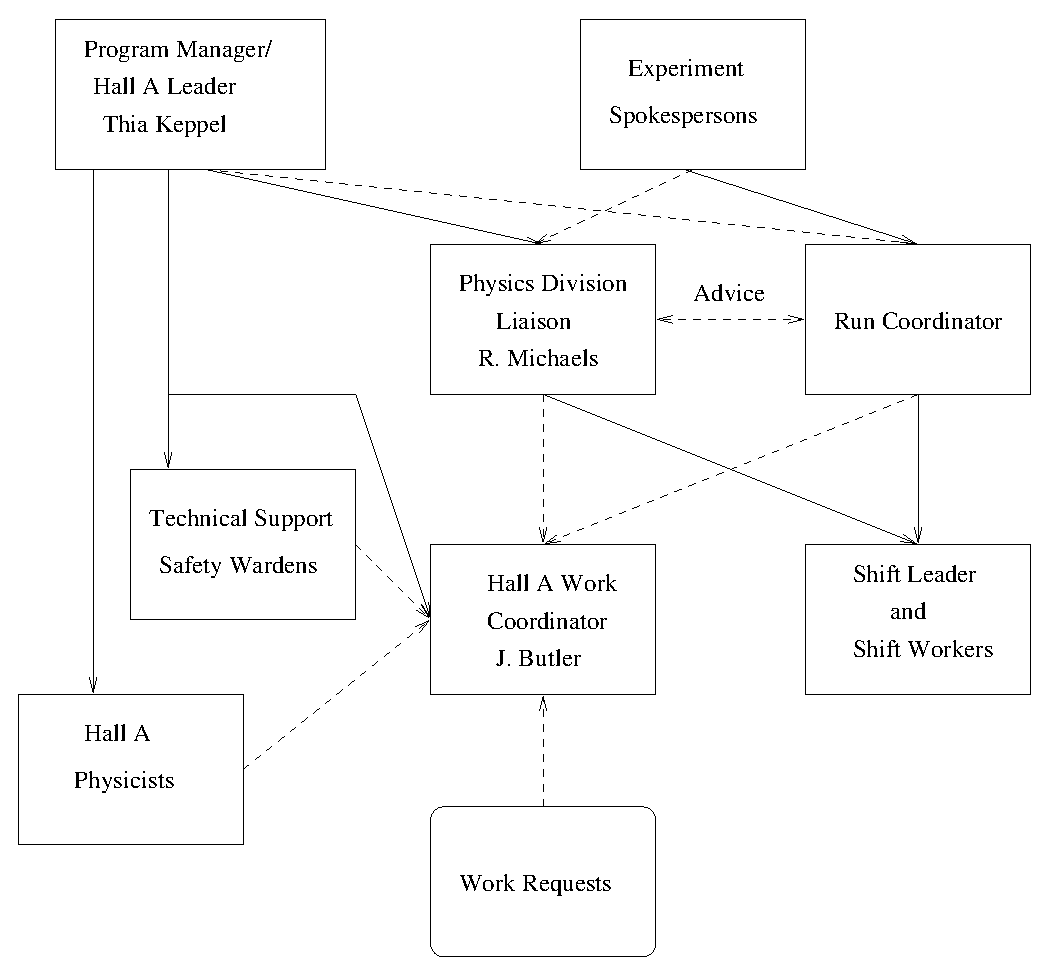
\includegraphics[width=\textwidth]{coo_HallAorg}
%
% Make a selection for a given Hall
%
%\centering{\special{psfile=coo_HallAorg hscale=70 vscale=80 hoffset=30 
%voffset=50}}
%
%\centering{\special{psfile=coo_HallBorg.eps hscale=70 vscale=80
%hoffset=30 voffset=50}}
%
%\centering{\special{psfile=coo_HallCorg.eps hscale=70 vscale=80 hoffset=30 
%voffset=50}}
\caption[Dummy caption.]{Functional Organization of the \HALL\ Team. Dashed
lines indicate information flow, solid lines indicate responsibility.}
\label{HALLCHART} 
%\label{fig:hallBchart}}
\end{figure}


\subsection{Run Coordinator}

 The Run Coordinator is the  immediate on-site manager of the experiment 
and is responsible for ensuring that the physics goals of the experiment 
are met. This individual is designated by the experiment spokespersons 
and approved by the Hall Leader.  The Run Coordinator shall ensure that 
the Hall Group Leader, Physics Division Liaison, and at least 
one Spokesperson are aware of all pertinent issues. The Run Coordinator
shall promote an environment in which the highest safety
standards are maintained.
{\bf All Run Coordinators must ensure that all of the JLab training necessary to perform 
their duties is up to date before their shift as Run Coordinator commences.}
The functions of the Run Coordinator  are: 

\noindent I. To manage daily operation of the experiment:

\begin{itemize}

\item to ensure that the run plan is clear to the shift workers.

\item to define the data quality appropriate for the goals of each shift.

\item to track the progress of the experiment.

\item to coordinate and schedule activities (e.g.,
Hall accesses) in order to optimize productivity.

\item to ensure that an experiment checklist is completed every 24 hrs during 
standby shifts.

\item together with the Physics Division Liaison, 
to ensure that the counting house is manned appropriately: i.e.,
sufficient personnel are present to safely carry out the experimental 
program or monitor the apparatus as needed.

\end{itemize}


\vspace{.25cm}

\noindent II. To coordinate interactions between JLab and the experiment. This
 entails:

\begin{itemize}

\item to ensure that the \HALL\ Group Leader and Experiment
Spokespeople are  aware of all necessary issues.

%G2P
%\item to coordinate with the various system leaders (Polarized target, beam polarimeter, data
%acquisition, and data analysis) and  schedule activities such
%as Moller runs, target anneals, thermal equilibrium
%measurements and Hall accesses to optimize productivity.
%G2P

\item informing the Program Deputy of the experiment's status and plans at 
a 7:45 AM program deputy/halls meeting in the MCC during the working week, and at an agreed
upon time on weekends or holidays.

\item representing the collaboration at the 8:00 AM daily summary meeting in the MCC
during the work week. 

\item attending the 1:30 PM Wednesday scheduling meeting in the MCC conference 
room to represent the collaboration and to present a report on the
preceding week.

\item remaining in the local area and being available by cell-phone/pager 
at all times.  (If temporarily unavailable the Run Coordinator must designate another 
qualified collaborator as a replacement.)

\item in conjunction with the Hall Work Coordinator, scheduling work by groups
outside the collaboration. 

\item interact with the Accelerator Program Deputy to plan and conduct
unscheduled activities.

%%G2P
%\item to maintain the ``Access Authorization List'' (a list of
%individuals who  are to be allowed entry to \HALL\ when the
%Hall is in Controlled Access or during maintenance) and  ensure that MCC has an up to
%date list.

\item in conjunction with the Hall Work Coordinator, scheduling
work by groups outside the collaboration. This work will
normally coincide with the scheduled  machine maintenance days.
This coordination requires a weekly meeting of these  two
individuals. The product of this meeting will include any necessary
updates to the ``Access  Authorization List''.

\item to be responsible for safe transition of the Hall to
Restricted Access in coordination with the Hall work
coordinator.

\item to provide an oral report at the weekly \HALL\
meeting\footnote{typically held at 1:30pm on Tuesday.} updating the
experimental progress to the collaboration.


\end{itemize}

\noindent III. To submit a written report to the Hall Leader which includes
run time statistics and a description of any significant problems with the 
Hall instrumentation.


\subsection{Physics Division Liaison}

Broadly speaking, the Physics Division Liaison to the experiment 
is a \HALL\ staff member selected by \HALLLEADER\
to oversee the hall's interests with respect to personnel and equipment 
protection.\footnote{The responsibilities described here correspond 
to those of the Physics Division Liaison during
the operating phase of the experiment as outlined in the
EH\&S Manual Chapter 3120/Glossary.} 
This is true for all four halls. However, the role of
the Physics Division Liaison may include other responsibilities
depending upon the experiment and other factors. His/her responsibilities
include:
\begin{itemize}
\item Oversee that proper rules of safety are carefully followed in the 
conduct of the experiment.
\item Approve a Hall status change to Restricted Access in coordination
with the Hall Work Coordinator.
\item Training verification of shift workers via JList software.
\item Together with the Run Coordinator, 
ensure that the counting house is manned appropriately: i.e.,
sufficient personnel are present to safely carry out the experimental 
program or monitor the apparatus as needed.
\end{itemize}  

\subsection{Hall Work Coordinator}

The Hall Work Coordinator's responsibilities are: 

\begin{itemize}

\item  to act as the {\bf single point of contact for all work in the hall.}

\item to determine if the scheduled activities in the hall can be done safely.
These activities shall be coordinated with the Physics Division Liaison
and the Run Coordinator.   Tasks should also be inputted into the work task
lists \url{http://www.jlab.org/listsites/}.

\item to ensure that workers are properly trained, are familiar with all
significant hazards, and are aware of all applicable work control
documents associated with the project. 

\item in coordination with the Physics Division Liaison, 
ensure that the hall apparatus is made safe before giving permission to
make a transition to Restricted Access (e.g., turn off unused magnets,
install protective shields as needed, fulfill specific requirements in the
ESAD, etc.).

 
\end{itemize}

\subsection{Shift Leader}

Each shift is led by a Shift Leader. The selection of shift leaders
is the responsibility of the Run Coordinator and Physics Division Liaison.
The  Shift Leader has the following responsibilities: 

\begin{itemize}

\item to carry out the scientific program planned for the shift in a safe
and efficient manner.

\item to ensure that the logbook contains a complete and accurate
description of the events and actions which occurred during the shift.

\item to serve as primary contact between the machine control center (MCC) and
experiment personnel.

\item  to oversee that hall equipment is operated properly.

\item to ensure the shift checklist is performed every eight hours on operating
shifts.

\item to ensure that equipment malfunctions are properly labeled and
locked-out if necessary and to communicate this to shift personnel and 
subsystem experts.

 \item to note in the logbook when workers from outside groups (such as survey 
and alignment) stop by the counting house before entering the hall when in 
Controlled Access. Furthermore, to confirm that these workers have
communicated with the Run Coordinator and the Hall Work Coordinator.

\item to coordinate the response of the shift crew to any
emergency situation, including the notification of appropriate individuals as
outlined in the \HALL\ Emergency Response Guidelines (ERG).

\item  to ensure that in any emergency situation the 
experiment Physics Division Liaison, Run Coordinator, and Hall Leader 
are notified immediately.

\item to notify the Run Coordinator and the Hall Leader, if the hall is down due to equipment failure for more than four hours.


\end{itemize}

The Shift Leader has the following authority: 

\begin{itemize}

\item to assign tasks to the shift members as needed.

\item to request that the state of the hall be changed (Request for a
change to Restricted Access must be approved by the Physics Division
Liaison.)

\item to limit the number of people in the Counting House or hall 
if required to effectively and safely carry out the experiment.

\item to limit access to hall on-line computers if required to
effectively and safely carry out the experiment.

\item to authorize qualified personnel to make modifications in the experiment
configuration within the allowed parameters, as specified in the standard equipment
manual.

\item to authorize time accounting for the shift.

\end{itemize}

\subsection{Shift Member}

The responsibilities of each shift member are to:
\begin{itemize}

\item carry out the scientific goals of the shift in a safe and efficient
 manner under direction of the shift leader.

\item read the logbook to be aware of changes in goals, operating
parameters, and new documentation.

\item monitor the equipment for problems.

\item maintain adequate records of the progress of the shift.

\item be present before the start of each shift and 
coordinate current operating conditions with the previous shift.

\item keep all training up-to-date.

\end{itemize}

\subsection{Accelerator Operations Hall Liaison}

Each physics hall has an Accelerator Operator or Crew Chief assigned as a Hall Liaison. 
The Hall Liaison helps to facilitate information exchange between the
experimenters and the MCC Operations Group, both in advance of and during
actual experiments. The Hall Liaison, among other things, is responsible 
for making sure that experiment-specific information, procedures and requirements 
are available to all other operators and Crew Chiefs so that beam delivery can proceed efficiently. 

\subsection{Accelerator Physicist Liaison}

The Accelerator Physicists Experiment Liaison serves as the primary contact on hall beam physics issues 
for the Physics, Accelerator and Engineering Divisions. This liaison owns the process of establishing 
physics quality beam to the experiment including developing beam optics configurations capable of 
meeting the experiments requirements, identifying tools needed to diagnose, monitor and verify 
beam performance during the experiment as well as developing beam startup, setup and commissioning 
plans. The \HALL\ liaison is \AccPhysLiaison\ .


\subsection{Engineering Liaison}

Each experiment conducted at JLab will be evaluated to determine if its complexity requires facilitation 
with the Engineering Division to help ensure a successful outcome.  Experiments that require 
facilitation will be assigned an individual from the Engineering Division to act as liaison 
between the Division and the associated Experimental and Physics Division staff. The liaison 
acts as a single point contact in order to facilitate information exchange 
between the experimenters and those in the Engineering Division responsible for, 
but not limited to, the systems requirements, design, scheduling, fabrication, 
installation, testing, documentation, and budgeting. Ideally, the liaison 
is aware of all work conducted by Engineering for the experiment and ensures 
the appropriate resources are defined and allocated. Any issues and/or concerns are identified, 
documented, and tracked.

For the current run period, the review found that no such liaison was required. 


%******************************************************************************
\section{Operating Procedures}

\subsection{Shift Routines}

There are two types of shifts for active hall experiments:
Operating and Standby. Operating shifts are the normal status
when beam is available for the experiment. Standby shifts are periods 
designated by the Run Coordinator when beam is not available or not in
use in the hall and none of the equipment, except for the target, requires
continuous monitoring. Standby status may result from normal operational
planning or from abnormal conditions such as a major down time due to
equipment failure.


\subsubsection{Operating Shifts}

During operating shifts, 24 hour occupation of the counting house area will 
be maintained by crews of at least two persons
\footnote{\label{fn2}The readiness review committee may require more 
personnel depending on the complexity of the experiment. Two people are 
the minimum required for safe operations.} 
in 8 hour shifts. One person per shift is designated as the Shift Leader.

The number of persons assigned to a shift will depend on the tasks assigned 
during the shift. A shift schedule will be posted in the Counting House 
listing the times and names of personnel on shift and identifying the 
Shift Leader and Run Coordinator, cell 876-1787. The shift schedule may be available at 
an experiment-specific website. The Run Coordinator may also designate 
and supervise other teams for duties such as offline analysis.

\subsubsection{Standby Shifts}

During Standby shifts, shift personnel are not required to be on site at 
JLab but must be available through telephone contact to come in if they
are needed.  Monitoring the target system can require the presence of a
Target Operator during a standby shift.  The Target Operator then also
acts as Shift Leader.  The Run Coordinator will ensure that the shift
checklist is executed at least once every 24 hours.

\subsubsection{Operations Turnover}
The electronic log book, accessible from the web, is a very effective means 
of remotely obtaining information about experimental operations. This allows 
experimenters to log in remotely and view all log book 
entries prior to commencing their shift.
Information which can only be recorded in the paper log book, should be
noted accordingly, point to in the electronic logbook, and communicated between incoming and outgoing shift 
personnel directly.

Efficient and effective shift changeovers during experiment operation 
are enhanced by overlapping shifts. Therefore, whenever possible, shift leaders 
and workers are scheduled in shifts that are staggered by four hours, leading 
to an overlap of half a shift.  If this is not the case, shift members must show
up ten minutes prior to shift start (and plan to stay ten minutes after) for the
purpose of information exchange to those taking over the same tasks.
In all cases incoming shift leaders must discuss the experiment and Hall status with the
outgoing shift leaders.

\subsubsection{Timely Orders to Operators}
The initial run plan is the responsibility of the Run Coordinator and
shall be clearly recorded in the log book. This plan specifies
the tasks to be performed in the next 48--72 hours, including
any special conditions or data runs, updated documentation and its
location and/or alternate plans. Any changes to the run plan shall
be recorded in the log book and the white board in the counting house.

\subsubsection{Operator Aid Postings}
The day-to-day schedule, contact instructions for key personnel, and 
any other information relevant to current activities are located
on the white board in the Counting House. Shift personnel should
consult the white board, especially at the beginning
of their shift, to be aware of any updates to current running conditions.

Information pertaining to daily activities in \HALL\ must be posted on the 
bulletin board or written on the white board at the entrance to the hall.

\subsection{Hall Access}

Work in designated radiation 
areas will be carried out in accordance
with the JLab RadCon Manual. In particular, no material 
may be removed from the hall after beam delivery
without proper approval from
the RadCon Group.
During operations, no one is allowed in the hall 
without either being accompanied, or informing shift personnel
and checking in on a regular basis. 
%This rule applies at 
%all times regardless of the access state of the hall. 
 
During a running experiment the hall will normally be in Beam Permit. When 
temporary access to the hall is needed the Shift Leader can ask the MCC to 
bring the hall to Controlled Access. If long term access to the hall is
required, the Shift Leader may request the hall be brought to Restricted
Access. Such a request requires prior approval from the Physics Division
Liaison, while the actual transition will be supervised by the Hall Work
Coordinator.

Restricted Access is a state where  delivery of beam and/or RF power is not 
permitted, and entry to and exit 
from the hall is not controlled by the Personnel Safety System. This is the 
normal state of the hall when the accelerator is off and no experiments are 
running. Access is ``restricted'' only in the sense that the hall is not open 
to the general public. Well-defined check-list procedures are to
be followed whenever the hall is brought to and from Restricted Access.

Restricted Access is the period when all major work must be completed in the
hall. Consequently, all activities require advanced planning and must be 
scheduled for resources and safe operation. In order to streamline the 
activities in the hall and ensure everyone
has ready access to the current status and requirements for work, there
are two important resources: 
\begin{itemize} 
\item Single point of contact, which is the ``Hall Work Coordinator''
\item Information board at the entrance to the hall
\end{itemize}
All work must be scheduled through the Hall Work Coordinator. The content 
on the information board is the responsibility of the hall safety wardens 
and the Hall Work Coordinator. The information board will contain all critical 
information required for safe entry into the hall. This information will
include a succinct, one page safety summary covering the hall's current
safety hazards and mitigating measures (to be read by all persons working
in the hall), active Operational Safety Procedures (OSPs) and Temporary
Operational Safety Procedures (TOSPs), required temporary work permits 
(e.g., Radiation Work Permits), current activities in the hall, points of 
contact, and required training and safety equipment.


\subsection{Collaboration Request for Laboratory Resources}

The collaboration may request additional services from Accelerator
Division through the Accelerator Division Liaison, \ACCDIVLIAISON.  Alternatively,
the collaboration may also request additional services from hall personnel 
through the Physics Division Liaison, \PHYSDIVLIAISON. These requests 
should be noted in the logbook. Some requests may require that an
OSP, or TOSP be developed.

Major, abnormal, or unanticipated configuration modifications such as stacking 
or movement of significant shielding, unanticipated vacuum work, unanticipated
beam line modifications, the replacement of a wire chamber, etc., require 
approval of the \HALL\ Leader, \HALLLEADER\ 
\footnote{\label{fn1}Configuration changes as outlined above can affect site
boundary dose and the production of airborne radioactivity. They require
consulting with RadCon or EH\&S personnel, as appropriate.}, and the use of 
appropriate personnel. The Hall Leader may require that a OSP, or 
TOSP be prepared.

\subsection{Scheduling of Work by Outside Groups }

Work in the hall that is to be performed by groups outside the collaboration 
such as survey and alignment, plant services, air conditioning , etc., 
must be scheduled so that it does not 
endanger personnel or equipment or interfere with the experiment.
Non-emergency activities by these groups should be
scheduled to coincide with the planned accelerator maintenance periods. 
To maximize efficiency, the Run Coordinator (representing the collaboration)
and the Hall Work Coordinator (representing \HALL) will concur
on work scheduling.
The Hall Work Coordinator's job is to 
coordinate activities in the hall so that work can take place smoothly 
and safely and to insure that multiple activities do not interfere. 

The Work Coordinator and the Run
Coordinator will meet as needed to plan the work
scheduled for the upcoming maintenance period.
The product of this meeting will be
a list of work in the hall, the required access state of the
hall (Controlled or Restricted), appropriate work 
control documents, and educational or other
safety measures (such as escorts) that are needed.

The ATLis should be used for coordinating the cross divisional work activities
\url{http://www.jlab.org/listsites/}. 

\subsection{Control of Equipment and System Status}
The operation of the standard experimental equipment is documented in the 
\HALL\ Standard Equipment Manual.
This document includes information on the
normal response to alarms and equipment malfunctions.
 
The ESAD and \HALL\ Standard Equipment Manual lists 
the authorized subsystem experts. This list may be amended as necessary to 
reflect personnel and training changes with the 
authorization of the subsystem expert. A copy of these 
amendments will be attached to the main document and kept in the
Counting House.

All general equipment installation, maintenance, and testing activities 
are to be carried out in accordance with the JLab EH\&S Manual.

\subsection{Equipment Labeling}
The experiment and hall equipment shall be properly labeled so 
it can be quickly identified by both shift and maintenance personnel.
Proper labeling helps prevent incorrect operation or modification of
equipment by non-experts and facilitates proper and efficient operation by
qualified personnel. Labeling also increases the likelihood that 
proper procedures will be followed in case of emergency.

Improper labels should be corrected immediately if possible.
Otherwise, the Shift Leader should be notified so that correct 
labeling can be requested from the qualified expert.


\subsection{Independent Verification}
	
The Run Coordinator will provide the shift crew with a set of 
measures for checking the quality of the experimental data.  
The up-to-date \HALL\ shift 
checklist (and instructions) shall be made available to shift personnel
at hall-specific sites on the data acquisition  computers.
The checklist will be completed at least once per shift during operating 
shifts and once per day during standby shifts. Additional items may be 
added to the list by the Run Coordinator or subsystem experts.

The \HALL\ work coordinator
provides more general check lists for closing the experimental Hall and 
conditions when the Hall is used as an accelerator dump.

\subsection{Logkeeping}

Shift personnel will update the electronic
logbook, which serves as the record of the experiment. 
The quality of the information recorded in the logbook 
determines the utility of the data.
All data recorded electronically
will be referenced in the  computer 
logbook with the appropriate run number and run information. All 
relevant activities are to be recorded, including 
all changes of experiment conditions and equipment failures.

Checklists performed using \HALL-specific forms should also be scanned 
into the computer logbook when completed. The completed paper forms should 
be stored in a binder in the counting house.  All deviations from normal 
operating parameters shall  be recorded in the logbook. 

The computer logbook will also serve as the primary reference for the
determination of the operational efficiency of the experimental apparatus in
the Hall. As such it is essential that it provide an accurate record of the 
capability of the equipment to carry out the intended research program. 
Finally, the computer logbook is the place of record for all safety issues and 
introductions of new or updated documentation and procedures.


\appendix

%
% comment out the appropriate file 
%
% Include here Hall dependent operation procedures
%
\newpage
\section{Special Procedures for \HALL}

Beyond the information covered in the Hall A standard equipment manual,
two operational safety proceedures have been written.
OSP-43091
provides safety information about the DVCS detector setup.  OSP-43679 provides
safety information about the new Hall A raster system.

% Include here experiment dependent operation procedures
%
\newpage
\section{Special Procedures for \EXPTS}

Each shift requires a shift leader and, if the cryotarget is cold, a cryotarget 
operator.  A third person on shift is extremely useful, but not required. The shift leader 
has the standard
duties of shift leader to ensure proper data taking, log all activity, and to fill out
the Beam Accounting form. The cryotarget operator should focus on cryotarget
operation. Training is arranged by Jian-Ping Chen. The shift leader or third
shift worker will run the DAQ and online analysis codes.
This run period uses the "standard" Hall A equipment whose
use and safety procedures are documented in the Hall A OSP (Operation Safety
Procedures) available from the Hall A web page.

\newpage
\section{Signature Sheets}

After reading this document, as well as the ESAD, RSAD, and ERG, workers need to sign
the signature sheet located in the "yellow binder" of the experiment specific documents.
This binder can be found in the \HALL\ counting house and in the MCC.


%\input{coo_hallb_appendix.tex}
%\input{coo_hallc_appendix.tex}


\end{document}

%
% Here you can find the correspondences between the simple Fermilab outline 
% and our beautiful COO.
%
%Chapter I: Operations Organization and Administration
%
%--> our Chapter II Organization and Administration
%
%
%Chapter II: Shift Routines and Operating Practices
%
%--> our 3.1 Shift Routines
%
%
%Chapter III: Control Room Activities
%
%--> our 2.4 Shift Leader, 2.5 Shift Member, and 3.1 Shift Routines
%
%Chapter IV: Communications
%
%--> our Chapter 2 Organization and Administration, our 3.1.3 Operations 
% Turnover, 3.1.4 Timely Orders to Operators, and 3.1.5 Operator Aid Postings
%
%
%Chapter V: Control of On-shift Training
%
%--> our Introduction,  Chapter I Shift Personnel Training, and 2.2 Physics
% Division Liaison
%  
%
%Chapter VI: Investigation of Abnormal Events
%
%--> our JLab Emergency Response Plan, 2.1 Run Coordinator, 2.2 Physics
% Division Liaison, and 2.4 Shift Leader 
%
%
%Chapter VII: Notifications
%
%--> our JLab Emergency Response Plan, 2.1 Run Coordinator, 2.2 Physics
% Division Liaison, and 2.4 Shift Leader 
%
%
%Chapter VIII: Control of Equipment and System Status
%
%--> our 2.3 Hall Work Coordinator, 3.2 Hall Access, 3.4 Scheduling of Work
% by Outside Groups, and 3.5 Control of Equipment
%
%
%Chapter IX: Lockouts and Tagouts
%
%--> our EH&S manual, chapter 6110
%
%
%Chapter X: Independent Verification
%
%--> our 3.6 Independent Verification
%
%
%Chapter XI: Logkeeping
%
%--> our 3.7 Logkeeping
%
%
%Chapter XII: Operations Turnover
%
%--> our 3.1.3 Operations Turnover
%
%
%Chapter XIII: Operations Aspects of Facility Chemistry and Unique Processes
%
%--> our 2.3 Hall Work Coordinator, and 3.2 Hall Access
%
%Chapter XIV: Required Reading
%
%--> our Preface and Introduction
%
%
%Chapter XV: Timely Orders to Operators
% 
%--> our 3.1.4 Timely Orders to Operators
%
%
%Chapter XVI: Operations Procedures
%
%--> our Chapter 3 Operating Procedures
%
%
%Chapter XVII: Operator Aid Postings
%
%--> our 3.1.5 Operator Aid Postings
%
%
%Chapter XVIII: Equipment and Piping Labeling
%
%--> our 3.5.1 Equipment and Piping Labeling











